\documentclass[11pt]{article}
\usepackage[margin=1in]{geometry}
\usepackage{amsmath,amssymb,amsthm,mathtools,bm}
\usepackage{graphicx,booktabs,longtable,array,microtype,enumitem}
\usepackage[authoryear,round]{natbib}
\usepackage[colorlinks=true,allcolors=blue]{hyperref}
\newtheorem{theorem}{Theorem}
\newtheorem{proposition}[theorem]{Proposition}
\newtheorem{lemma}[theorem]{Lemma}
\newtheorem{corollary}[theorem]{Corollary}
\theoremstyle{definition}
\newtheorem{definition}[theorem]{Definition}
\theoremstyle{remark}
\newtheorem{remark}[theorem]{Remark}
\newcommand{\R}{\mathbb R}
\newcommand{\E}{\mathbb E}
\newcommand{\PP}{\mathbb P}
\newcommand{\ip}[2]{\langle #1,#2\rangle}
\newcommand{\norm}[1]{\lVert #1\rVert}
\newcommand{\Th}{\Theta}
\newcommand{\one}{\mathbf 1}
\newcommand{\tn}{t_n}
\newcommand{\pr}{\textsc{Proved}}
\DeclareMathOperator{\rank}{rank}
\DeclareMathOperator{\dist}{dist}
\DeclareMathOperator{\vecop}{vec}
\DeclareMathOperator{\TV}{TV}
\DeclareMathOperator{\KL}{KL}
\setlength{\emergencystretch}{3em}
\setlist{nosep}
\graphicspath{{figures/}}
\bibliographystyle{plainnat}

\title{Contact Orders and the Fragility of Honest Tensor Inference}
\author{Research draft for author review}
\date{7 September 2026}
\begin{document}
\maketitle
\begin{abstract}
A linear functional of a tensor coefficient can have a vanishing first-order derivative when restricted to a rank-constrained model. We study the resulting inference problem in Gaussian tensor regression with fixed ambient dimension. At an original-mode rank-one signal, we classify the local modulus for every tensor-train rank-cap profile: cuts constrained to rank one partition the modes into blocks, and the first nonzero block degree of the loading determines the contact order $q$. The optimal pointwise expected length among intervals honest over the entire class is of order $(\sigma/\sqrt n)^q/\lambda^{q-1}$, where $\lambda$ is signal magnitude. The classification includes examples with singular internal rank constraints. In a known Frobenius neighborhood of radius $\eta$, the optimal order acquires the term $\eta\wedge(\sigma/\sqrt n)$. We construct a computable interval using a Gaussian confidence ball, an HOSVD pilot, and all block orders, with an exact extension to unknown variance. Simulations recover the predicted exponents and distinguish exact-boundary Wald calibration from locally honest inference, while documenting substantial conservatism of the proposed interval. The contribution is a tensor-specific classification and sensitivity calculation; generic higher-order inference, modulus lower bounds, and tensor tangent geometry are established tools.
\end{abstract}
\noindent\textbf{Keywords:} confidence intervals; tensor train; local modulus; singular inference; model approximation; higher-order contact.

\section{Introduction}
Structural restrictions can reduce uncertainty about a regression functional by more than a variance constant. Consider a four-way coefficient $B\in\R^{2\times2\times2\times2}$ whose TT rank caps are $(1,2,1)$. The outer rank-one cuts force a product of blocks of dimensions $(2,4,2)$. At $B_0=\lambda E_{0000}$, the coordinate functional $B\mapsto B_{1111}$ changes only when all three blocks change. A perturbation of Frobenius size $t$ can change this functional by order $t^3/\lambda^2$. This raises a statistical question: can an interval exploit that cubic behavior while retaining coverage over the whole rank-constrained class, including neighboring rank strata?

Existing theory makes a simple higher-order calculation insufficient as a contribution. Functional inference under degeneracy, including corrected bootstrap and minimum-distance methods, is well developed \citep{chenfang2019,bei2026}. Tensor inference with nondegenerate tangent alignment also has strong guarantees \citep{xu2025,maxia2024}. What requires a separate calculation here is the local modulus across a specified collection of TT constraints and the corresponding expected length under global honesty. In addition, structural rank restrictions may be approximate, and a small coefficient departure can be larger than a higher-order inferential scale.

We therefore study a deliberately explicit experiment: independent isotropic Gaussian designs, independent Gaussian regression errors, and a fixed-dimensional coefficient in a bounded TT rank class or a known neighborhood of that class. The estimand is a fixed linear functional of the coefficient, not an individual TT core, a training-trajectory statistic, or an unobserved neural-network parameterization. Our main objective is to classify the best expected interval length at rank-one coefficients subject to coverage for every coefficient in the declared class. We allow unknown error variance but do not claim inference when ambient least squares is unavailable.

Three obstacles distinguish the calculation from a direct delta-method exercise. First, a path in an enclosing product model may violate an internal TT rank cap, so a lower modulus bound requires an actually feasible tensor path. Second, a confidence interval calibrated at the exact boundary can fail under statistically indistinguishable local changes, as Figure~\ref{fig:activation} illustrates. Third, the fitted loading projections have lower-order components even when the true ones vanish; these terms and the event of poor pilot localization must be controlled to bound expected length.

The construction uses the cuts whose rank cap equals one to partition the tensor chain. Orthogonal loading components are graded by the number of blocks perpendicular to the signal. The smallest nonzero degree determines the modulus exponent. Within-block sums of two elementary products provide feasible witness paths despite the remaining TT constraints. Confidence-ball inversion then supplies global coverage, while a graded product bound makes the calculation explicit. In the four-way example this recovers cubic inference. A six-way example with a proper singular internal rank constraint has the same cubic order, demonstrating both the scope of the classification and the limited role of that singularity.

The paper makes three claims, each proved in the appendix:
\begin{enumerate}
 \item Section~\ref{sec:theory} classifies local contact and optimal honest expected length at rank-one signals for arbitrary positive TT cap profiles. It also shows that slack at every cut restores first-order contact for every nonzero loading.
 \item Theorem~\ref{thm:length} determines the additional length required by a known structural approximation allowance and identifies departures that cannot be detected but invalidate exact-model lengths.
 \item Section~\ref{sec:method} gives a computable, globally honest interval that attains these orders without selecting the contact order. The experiments test the exponents, local coverage distinction, and approximation sensitivity.
\end{enumerate}

\begin{figure}[t]
\centering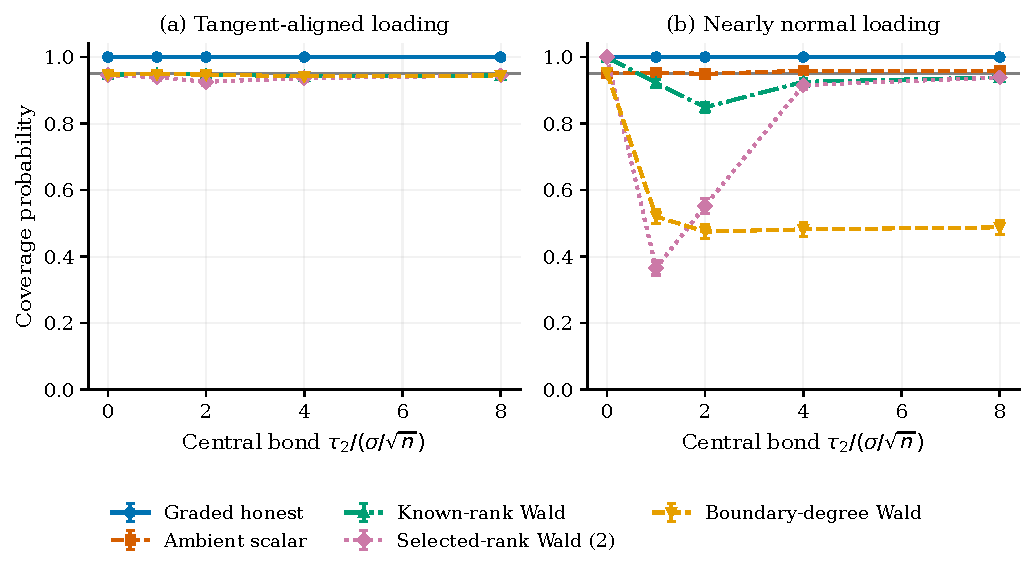
\includegraphics[width=\textwidth]{activation.pdf}
\caption{Exact-boundary calibration can fail under a local change in the central TT bond. Four binary modes have caps $(1,2,1)$, $n=2048$, $\lambda=3$, and $\sigma=0.2$; the path and two fixed loadings are specified in Section~\ref{sec:experiments}. Points use 2,000 replications with Wilson 95\% Monte Carlo intervals; the horizontal line is nominal coverage 0.95. ``Selected-rank Wald (2)'' uses the prespecified threshold multiplier two.}\label{fig:activation}
\end{figure}

\section{Related work and the scope of the contribution}
\paragraph{Degenerate functionals and singular tests.}
\citet{chenfang2019} develops second-order functional inference and explains ordinary-bootstrap failure; higher-order extensions are explicitly discussed. \citet{dufour2025} studies locally singular polynomial Wald restrictions. \citet{pillaimeng2016} gives the exact Gaussian monomial Wald law, including the cubic $\chi_1^2/9$ case. \citet{bei2026} constructs uniformly valid minimum-distance inference under degeneracy and discusses extensions beyond a nonsingular Hessian. These results preclude novelty claims based solely on a cubic delta method or a nonstandard Wald limit. Our explicit local Wald calculation is a supporting specialization of that literature.

\paragraph{Moduli, curved models, and model neighborhoods.}
The connection between honest interval length and between-class moduli is central to \citet{cailow2004}. Its lower-bound logic applies to singleton evaluation classes and does not require a new tensor information inequality. \citet{andrews2016} already obtains conservative inference from curved-model geometry. Model-misspecification sensitivity is studied by \citet{bonhomme2022}, and bias-aware intervals and efficiency comparisons by \citet{armstrong2021,armstrong2023}. Our neighborhood calculation uses the elementary modulus sandwich; the specific input is the classified TT contact order. We do not claim a new general theory of robust confidence intervals.

\paragraph{Rank uncertainty and tensor inference.}
\citet{carpentier2018} shows that rank-adaptive matrix confidence sets can exist, with feasibility depending on the observation and noise experiment. \citet{armstrong2026} allows weak factors in panel inference. Thus rank uncertainty is not a universal impossibility mechanism. In regular tensor settings, \citet{xu2025} and \citet{maxia2024} obtain functional Gaussian limits under signal, initialization, and nondegenerate alignment conditions. Their dimensions can increase, and their regular-regime results are stronger than the fixed-dimensional analysis here in that respect. We address a different boundary regime rather than improving their sample complexity. \citet{xia2022} also establishes important tensor inference results without a universal need for debiasing.

\paragraph{Tensor geometry, estimation, and computation.}
\citet{kutschan2018} characterizes TT tangent cones, and \citet{yang2025} gives first- and second-order variational formulas for determinantal tensor formats. Higher block-degree spans for product varieties appear in the osculating geometry of \citet{araujo2019}. We use that grading and verify feasible lower-bound paths inside the additional TT constraints. TT regression estimation and algorithmic guarantees are already supplied by \citet{qin2025}; oracle tensor regression under separation is studied by \citet{wang2025}. The spectral-norm hardness observation in Proposition~\ref{prop:hardness} inherits the result of \citet{hillarlim2013}; it is not an independent complexity theorem.

\paragraph{Modern tensor models and other inferential targets.}
Tensor regression networks \citep{kossaifi2020}, global rank-adaptive TT adapters \citep{metatt2026}, and statistical rank allocation for LoRA \citep{gao2026} motivate attention to rank restrictions. Their architectural or optimization targets should not be conflated with the present population coefficient. Tensor conformal completion \citep{suncheng2026} and the recent dual-channel tensor framework \citep{dual2026} further demonstrate that tensor uncertainty quantification is already an active area. Predictive intervals and structure-comparison guarantees in those experiments do not determine the honest length studied here.

The literature assessment is current through 7 September 2026. The accompanying novelty matrix records mathematical settings, assumptions, guarantees, versions and differences for 25 comparisons, with a retained review of all 18 supplied PDFs. No reviewed source states the cap-profile classification and structural-neighborhood length formula in the form proved below. That observation supports a candidate contribution, not an assertion that all overlapping unpublished results have been excluded.

\section{Statistical experiment and inferential objective}\label{sec:problem}
\subsection{Data, loss, and structural parameters}
Fix an integer $K\ge2$ and positive mode dimensions $d_1,\ldots,d_K$, and set $p=\prod_{k=1}^Kd_k$. We observe independent pairs $(X_i,Y_i)$, where $X_i\in\R^{d_1\times\cdots\times d_K}$, $x_i=\vecop(X_i)$, and
\begin{equation}\label{eq:model}
 x_i\stackrel{\rm iid}{\sim}N_p(0,I_p),\qquad
 Y_i=x_i^\top b+\varepsilon_i,\qquad
 \varepsilon_i\stackrel{\rm iid}{\sim}N(0,\sigma^2),\quad b=\vecop(B).
\end{equation}
Designs and errors are independent. Vectorization preserves the mode order throughout; the implementation uses C order. There are no latent random structural factors in this experiment. TT cores are nonunique parameterizations of the coefficient and are not inferential targets. Write $P_{B,\sigma}^{(n)}$ for the joint law of all observations. The noise scale is either known or estimated as specified later.

The half-squared loss is $\ell(B;x,y)=(y-x^\top b)^2/2$. Its risk and empirical risk are
\[
 R(B)=\E_{B^\star,\sigma}\ell(B;x,Y),\qquad
 R_n(B)=\frac1n\sum_{i=1}^n\ell(B;x_i,Y_i).
\]
In \eqref{eq:model}, $R(B)-R(B^\star)=\norm{B-B^\star}_F^2/2$, so the coefficient is identifiable even before structural restrictions. Ambient OLS is the unique empirical minimizer for full-column-rank design. Our structured pilot is a rank-one HOSVD of OLS in specified blocks, not an assertion that a globally optimal constrained least-squares tensor can be computed.

For the prefix unfolding $B^{[k]}\in\R^{(d_1\cdots d_k)\times(d_{k+1}\cdots d_K)}$, define $r_k(B)=\rank(B^{[k]})$. Given positive integer caps $\bar r=(\bar r_1,\ldots,\bar r_{K-1})$ and $M>0$, let
\begin{align*}
 \Th_0&=\{B:r_k(B)\le\bar r_k\text{ for }1\le k<K,\ \norm{B}_F\le M\},\\
 \Th_\eta&=\{B:\norm{B}_F\le M,\ \dist_F(B,\Th_0)\le\eta\},\qquad\eta\ge0.
\end{align*}
These sets are closed and bounded. The caps and the allowance $\eta$ are specified independently of the data. All actual ranks below the caps are allowed, including simultaneous rank drops. A known $\eta$ is a sensitivity parameter bounding coefficient approximation; it is not a contamination proportion or a data-derived certificate.

\subsection{Target, honesty, and regime}
Fix a nonzero deterministic loading $A$ and target $\psi_A(B)=\ip{A}{B}$. Examples are individual entries or prespecified weighted contrasts. The evaluation metrics are coverage and expected interval length, not support recovery or generalization error of a trained feature map. Honesty means
\[
 \inf_{B\in\Th_\eta}\PP_{B,\sigma}\{\psi_A(B)\in I\}\ge1-\alpha,
 \qquad 0<\alpha<1/2,
\]
with the infimum also over $\sigma>0$ for a procedure that does not know $\sigma$. A short interval at one point is only useful for this objective if coverage holds over the declared class. No regularity, equivariance or asymptotic-linearity condition is imposed on competing intervals in the lower bound.

The length analysis fixes $K,d_k,\bar r,A$ and the signal directions, and evaluates rank-one points $B_0=\lambda\bigotimes_ku_k$ with $0<\lambda<M/2$. Constants are not dimension free. We assume $n\ge2p+2J+8$, where $J$ is the number of cap-one-induced blocks, and $\sigma/\sqrt n$ is sufficiently small relative to $\lambda$. The latter condition keeps the local alternatives away from zero signal. These restrictions are sufficient for the inverse-design moments used in the proof; finite-sample coverage alone needs only $n>p$ and full-column-rank design.

The roles of the assumptions are distinct. Original-mode rank one makes the within-block witness paths feasible with internal ranks at most two. The known cap-one cuts exclude the ambient directions responsible for slower inference. The norm cap provides compactness and an interior margin. Gaussian errors give exact chi-square and $F$ localization; isotropic random design gives the stated information distance and length moments. Conditional coverage permits other full-rank designs, but the displayed sharp rate calculation uses \eqref{eq:model}. No sparsity, observation contamination, dependent-noise validity, or growing-dimensional optimality is implicit in these assumptions.

\section{Contact order and honest expected length}\label{sec:theory}
Write $\mathcal C=\{k:\bar r_k=1\}$ and partition the ordered modes at these cuts into $J=|\mathcal C|+1$ consecutive blocks. Their dimensions are $D_1,\ldots,D_J$. At
\[
 B_0=\lambda u_1\otimes\cdots\otimes u_K,
 \qquad \norm{u_k}=1,\quad 0<\lambda<M/2,
\]
let $v_j$ be the product of the original factors in block $j$. Define $P_j=v_jv_j^\top$, $Q_j=I-P_j$, and the mutually orthogonal components
\[
 A_S=\left(\bigotimes_{j\in S}Q_j\bigotimes_{j\notin S}P_j\right)A,
 \qquad S\subseteq[J],
\]
where operators are applied in mode order. For $A\ne0$, define
\begin{equation}\label{eq:q}
 q(A,B_0,\bar r)=\max\{1,\min\{|S|:A_S\ne0\}\}.
\end{equation}
This definition treats a nonzero radial component as first order. It is unchanged by sign choices for the signal factors. Define the local modulus
\[
 \omega_{A,\eta}(t;B_0)=\sup\{|\ip{A}{B-B_0}|:B\in\Th_\eta,\ \norm{B-B_0}_F\le t\}.
\]

\begin{theorem}[Contact-order classification; \pr]\label{thm:contact}
Fix the dimensions, positive integer caps, unit factors, and nonzero loading $A$, with $q$ as in \eqref{eq:q}. There are positive constants $c,C,t_0$, depending on this fixed geometry, such that, for $0<t\le t_0\lambda$ and $\lambda+t<M$,
\begin{equation}\label{eq:modulus}
 c\frac{t^q}{\lambda^{q-1}}\le\omega_{A,0}(t;B_0)
 \le C\frac{t^q}{\lambda^{q-1}}.
\end{equation}
The upper inequality, after increasing $C$, holds for every $t>0$. If $A$ is a unit product across the blocks, equal to $v_j$ on inactive blocks and to an elementary original-mode product $w_j\perp v_j$ on exactly $q\ge1$ active blocks, then
\begin{equation}\label{eq:sharpconstant}
 \lim_{t/\lambda\to0}\frac{\lambda^{q-1}\omega_{A,0}(t;B_0)}{t^q}
 =q^{-q/2}.
\end{equation}
Here an elementary product uses factors from orthonormal bases whose first vectors are the $u_k$.
\end{theorem}

Only cap-one cuts determine the exponent. Internal caps constrain the feasible directions and the modulus constants, but permit a sum of two elementary products within each block. These paths attain the exponent even if the internal TT variety is singular. The block grading on the surrounding product variety is classical osculating geometry; our calculation determines which of these orders remain attainable inside the capped TT class.

For example, in six binary modes with caps $(1,2,2,2,1)$, the block dimensions are $(2,16,2)$. The middle four-mode block has a proper central matrix-rank constraint at most two, singular at a rank-one signal. At $B_0=\lambda E_{000000}$ and $A=E_{111111}$, $q=3$ and the constant in \eqref{eq:sharpconstant} is $1/(3\sqrt3)$. This example includes an internal singularity; it is not a claim that the singularity itself creates the cubic exponent.

\begin{proposition}[Slack at every cut; \pr]\label{prop:slack}
Let $B\in\Th_0$ have $\norm{B}_F<M$ and
\[
 \rank(B^{[k]})+1\le\bar r_k\quad\text{for every }k.
\]
For every $A\ne0$, $\omega_{A,0}(t;B)\asymp t$ for sufficiently small $t$. In particular, at an original-mode rank-one point, if every cap is at least two, no nonzero linear functional has a higher-order modulus.
\end{proposition}

This is an exponent statement with geometry-dependent constants. It does not assert that every honest interval must have the ambient efficient variance, or that growing-dimensional constants are harmless.

Let $\mathfrak I_{\eta,\alpha}$ be the measurable closed intervals satisfying coverage at least $1-\alpha$ for every $B\in\Th_\eta$ (and every $\sigma>0$ for unknown-noise procedures). Set
\[
 L_{\eta,\alpha}(B_0;\sigma)=\inf_{I\in\mathfrak I_{\eta,\alpha}}\E_{B_0,\sigma}|I|,
 \qquad \tn=\sigma/\sqrt n.
\]
The infimum is a statistical benchmark, without a computational restriction.

\begin{theorem}[Honest length and structural approximation; \pr]\label{thm:length}
Suppose $0<\alpha<1/2$, the fixed-geometry assumptions of Theorem~\ref{thm:contact} hold, and $n\ge2p+2J+8$. There is a sufficiently small geometry-dependent $c_0>0$ such that, for $\tn\le c_0\lambda$ and every known $\eta\ge0$,
\begin{equation}\label{eq:length}
 L_{\eta,\alpha}(B_0;\sigma)\asymp
 \frac{\tn^q}{\lambda^{q-1}}+(\eta\wedge\tn).
\end{equation}
Constants may depend on $\alpha,A$, dimensions, factors, and caps, but not on $n,\sigma,\lambda,\eta$ subject to the stated restrictions. The upper bound holds for the computable interval in Section~\ref{sec:method}, both with known and unknown noise variance.
\end{theorem}

By \eqref{eq:length}, when $q\ge2$ the exact-model rate survives a known approximation allowance only when $\eta\lesssim\tn^q/\lambda^{q-1}$. A coefficient perturbation much smaller than the ordinary noise scale can therefore destroy most of the gain. This is not resistance to contaminated observations: $\eta$ bounds the distance of the regression coefficient from the specified structural class. The neighborhood argument is general; its tensor-specific input is \eqref{eq:modulus}.

\begin{corollary}[Undetectable departures; \pr]\label{cor:pretest}
For a unit loading with $q\ge2$, let $s_n=\tn^q/\lambda^{q-1}$ and suppose $s_n=o(\eta_n)$ and $\eta_n=o(\tn)$. Then $B_n=B_0+\eta_n A$ belongs to $\Th_{\eta_n}$ for all sufficiently large $n$, $\TV(P_{B_n,\sigma}^{(n)},P_{B_0,\sigma}^{(n)})\to0$, and every interval honest over $\Th_{\eta_n}$ has expected length at $B_0$ at least $(1-2\alpha-o(1))\eta_n$. No rank pretest can make an $O(s_n)$ expected-length interval uniformly honest over that tube.
\end{corollary}

\subsection{Comparison with a single matrix constraint}
The six-mode example has cubic contact. In a single prefix unfolding with cap one, the same elementary loading is normal in both matrix factors and has quadratic contact. For a prefix cap two, the rank-one point has slack and has first-order contact. Thus none of the five individual prefix constraints alone yields the cubic exponent. This establishes a difference from any one such matrix envelope, not from all possible nonlinear matrix parameterizations or arbitrary collections of matrix constraints.

\begin{proposition}[Complexity of a leading constant; \pr]\label{prop:hardness}
Consider the three-block rank-one class in dimensions $(m_1+1,m_2+1,m_3+1)$, $B_0=\lambda e_0^{\otimes3}$, and a loading $A$ supported entirely on the three perpendicular subspaces. Let $T$ denote its $m_1\times m_2\times m_3$ coefficient array. Then
\[
 \lim_{t/\lambda\to0}\frac{\lambda^2\omega_{A,0}(t;B_0)}{t^3}
 =\frac{\norm{T}_{\rm inj}}{3\sqrt3},\qquad
 \norm{T}_{\rm inj}=\max_{\norm{x}=\norm{y}=\norm{z}=1}|\ip{T}{x\otimes y\otimes z}|.
\]
Consequently, when these dimensions vary, exact evaluation of this leading coefficient contains the tensor spectral-norm problem of \citet{hillarlim2013}.
\end{proposition}
This is a reduction to an existing hardness theorem. It neither proves a computational--statistical minimax gap nor precludes conservative polynomial-time intervals.

\section{A computable interval without contact-order selection}\label{sec:method}
Let $X$ have rows $x_i^\top$, $S=X^\top X$, and $z=S^{-1}X^\top Y$. For known $\sigma$, use
\[
 e=\sigma\sqrt{\chi^2_{p,1-\alpha}/\lambda_{\min}(S)}.
\]
For unknown $\sigma$ and $n>p$, set $\widehat\sigma^2=\norm{Y-Xz}^2/(n-p)$ and
\begin{equation}\label{eq:Fball}
 e=\widehat\sigma\sqrt{pF_{p,n-p;1-\alpha}/\lambda_{\min}(S)}.
\end{equation}
Both the known-noise radius and \eqref{eq:Fball} give $\PP(\norm{z-b}\le e\mid X)\ge1-\alpha$ for every full-rank design under the Gaussian error model. The Euclidean ball contains the exact ellipsoid; its radius can be conservative.

Reshape $z$ into the $J$ blocks and take its rank-one HOSVD approximation $\widehat B=\widehat s\bigotimes_j\widehat v_j$, with $\widehat s=\norm{\widehat B}_F\ge0$ and signs absorbed into the factors. Ties are resolved by a fixed measurable rule. This pilot need not satisfy the internal TT caps. Let $\widehat\Pi_\ell$ project onto the sum of block components with exactly $\ell$ perpendicular factors, and write $\widehat\Pi_{\le1}=\widehat\Pi_0+\widehat\Pi_1$. Put
\[
 \rho=\norm{z-\widehat b}+e+\eta.
\]
For $\rho<\widehat s/2$, define
\begin{equation}\label{eq:graded}
 H=\min\left\{\norm{A}_F\rho,
 \norm{\widehat\Pi_{\le1}A}_F\rho+
 \sum_{\ell=2}^J \binom{J}{\ell}^{1/2}
 \norm{\widehat\Pi_\ell A}_F
 \frac{\rho^\ell}{(\widehat s-\rho)^{\ell-1}}\right\}.
\end{equation}
Otherwise set $H=\norm{A}_F\rho$, including a zero pilot. The structured interval and the ambient projection are
\[
 I_s=[\ip{A}{\widehat B}\ \pm(H+\eta\norm{A}_F)],\qquad
 I_a=[a^\top z\ \pm e\norm{a}],\quad a=\vecop(A).
\]
Return $I=I_s\cap I_a$ if the intersection is nonempty, and the singleton $\{a^\top z\}$ otherwise. Intersecting uses the same confidence-ball event; there is no additional multiplicity charge. The empty-intersection convention matters only outside that event.

\begin{theorem}[Coverage and adaptation to contact order; \pr]\label{thm:procedure}
For every $B\in\Th_\eta$, the above interval has conditional coverage at least $1-\alpha$ for any full-column-rank design and independent homoskedastic Gaussian errors. Under the random-design assumptions and sample-size conditions of Theorem~\ref{thm:length},
\[
 \E_{B_0,\sigma}|I|\le C\left\{\tn^q/\lambda^{q-1}+\eta\wedge\tn\right\}.
\]
The algorithm requires the caps, loading, and known approximation allowance, but does not require the true factors, $\lambda$, or $q$.
\end{theorem}

The guarantee is rate optimal in $n$ with fixed geometry. Its constants include ambient dimension through localization and can be large. Evaluating the orthogonal components by all masks uses $2^J$ terms; no efficiency claim is made when the number of blocks increases. The theory does not cover $p\ge n$. In the one-block case the pilot is $z$ and the procedure reduces to an ambient ball projection.

\subsection{Why exact boundary calibration is insufficient}
For the four-way class with caps $(1,2,1)$, consider
\[
 B_{n,c}=\lambda(e_0+u_ne_1)\otimes(e_{00}+u_ne_{11})
                    \otimes(e_0+u_ne_1),\qquad u_n=c\tn/\lambda,
\]
and $A=E_{1111}$. Let $\widehat\psi=\ip{A}{\widehat B}$ for the three-block HOSVD pilot, and define the tangent plug-in standard error
\[
 \widehat{\rm se}=\sigma\sqrt{(\widehat\Pi_{\le1}a)^\top S^{-1}
                                      (\widehat\Pi_{\le1}a)}.
\]
\begin{proposition}[Local Wald experiment; \pr]\label{prop:wald}
With fixed $\lambda,\sigma>0$ and each fixed $c\ge0$, put $s_n=\tn^3/\lambda^2$. Under $B_{n,c}$,
\[
 \left(\frac{\widehat\psi}{s_n},\frac{\widehat{\rm se}}{s_n}\right)
 \xrightarrow{d}
 \left(\prod_{j=1}^3(c+Z_j),
 \left\{\sum_{j=1}^3\prod_{k\ne j}(c+Z_k)^2\right\}^{1/2}\right),
\]
where the $Z_j$ are independent standard normal variables, and $\psi_A(B_{n,c})/s_n=c^3$. At $c=0$, the interval $[\widehat\psi\pm z_{1-\alpha/2}\widehat{\rm se}/3]$ has limiting coverage $1-\alpha$, by \citet{pillaimeng2016}. Its coverage, taking first $n\to\infty$ and then $c\to\infty$, instead tends to
\[
 2\Phi(z_{1-\alpha/2}/3)-1,
\]
approximately $0.4865$ at $\alpha=0.05$. Ordinary Wald calibration has iterated limit $1-\alpha$.
\end{proposition}
This specializes known degeneracy phenomena and is not a separate priority claim. The result concerns the three-block pilot; the known-rank-one pilot at $c=0$ is a different estimator.

\section{Experiments linked to the theory}\label{sec:experiments}
\subsection{Design, estimators, and Monte Carlo uncertainty}
The primary design was recorded after the main derivations and before execution. It contains 81 settings, each with 2,000 independent replications, at nominal coverage 0.95. A separate, explicitly post-primary addendum contains 12 larger-sample settings to investigate finite-sample slope effects. Together these use 186,000 datasets and 1,410,000 method--functional interval evaluations. All random streams are determined by a master seed and a setting identifier. The full design, per-setting metadata, compressed replicate records, and analysis code accompany the paper.

For the Gaussian experiments we simulate the exact joint distribution of the sufficient statistics using Bartlett's Wishart construction. Specifically, if $S=LL^\top$, $G\sim N_p(0,I)$ and $V\sim\chi^2_{n-p}$ are independent of the design, then
\[
 z=b+\sigma L^{-\top}G,\qquad \widehat\sigma=\sigma\sqrt{V/(n-p)}.
\]
This has the same law as ambient OLS and its residual scale from $n$ Gaussian observations. Large values of $n$ therefore do not require storing an $n$ by $p$ matrix. The stress experiments instead generate the actual observations because their error laws are outside this construction.

The operational baseline with an exact finite-sample scalar guarantee is ambient OLS: $a^\top z\pm z_{.975}\sigma\sqrt{a^\top S^{-1}a}$, or its residual-$t$ version. We compare the graded interval with this baseline, ordinary HOSVD tangent plug-in Wald, the boundary-degree calibration, and a single-prefix-matrix envelope. The last method applies two-block graded inversion at the first available cap-one cut and otherwise uses ambient inference. It is a containing-model baseline, not a claim to optimize every possible unfolding method. Exact inversion of the nonconvex TT confidence region is a theoretical benchmark; the graded procedure computes an outer certificate rather than globally optimized endpoints.

For an interval $I^{(r)}$, reported coverage is $\widehat c=R^{-1}\sum_r\one\{\psi_A(B)\in I^{(r)}\}$ and its binomial Monte Carlo standard error is $\sqrt{\widehat c(1-\widehat c)/R}$. At $R=2000$ and $c=0.95$, this is 0.00487. Wilson 95\% Monte Carlo intervals are also reported, including at zero or full empirical coverage. Mean lengths have standard errors equal to their sample standard deviations divided by $\sqrt R$. At 2,000 successes out of 2,000, a zero plug-in standard error does not imply certainty: the Wilson interval is approximately $[0.9981,1]$.

\subsection{Contact orders and internal singularity}
We take $B_0=3E_{00\cdots0}$, $A=E_{11\cdots1}$, and $\sigma=0.2$. Three binary modes with caps $(1,1)$ give $q=3$. Four binary modes with caps $(1,1,1)$, $(1,2,1)$, $(2,1,2)$, and $(2,2,2)$ give $q=4,3,2,1$, respectively. Six binary modes with caps $(1,2,2,2,1)$ give the internally singular $q=3$ example. The primary sample sizes are 512, 2048 and 8192.

The mean-length slopes approach the predicted $-q/2$ exponents; Table~\ref{tab:slopes} reports both the primary and larger-$n$ estimates. The primary six-mode slope is $-1.776$, so those sample sizes alone should not be described as a precise confirmation of $-1.5$. The addendum uses $n=131072$ and $2097152$, with unchanged methods and tuning. Its six-mode slope is $-1.511$, while the four-way product slope is $-2.010$. Monte Carlo errors in the table describe uncertainty in simulated means, not error from approximating an asymptotic exponent.

\begin{table}[t]
\centering\small
\begin{tabular}{lrrrr}
\toprule
Profile & $p$ & Predicted & Primary & Large-$n$ (MCSE) \\
\midrule
Four-mode slack & 16 & -0.50 & -0.548 & -0.503 ($9.4\times10^{-6}$) \\
Four-mode two blocks & 16 & -1.00 & -1.071 & -1.003 (0.002) \\
Three-mode product & 8 & -1.50 & -1.563 & -1.504 (0.004) \\
Four-mode three blocks & 16 & -1.50 & -1.605 & -1.500 (0.003) \\
Six-mode singular & 64 & -1.50 & -1.776 & -1.511 (0.002) \\
Four-mode product & 16 & -2.00 & -2.136 & -2.010 (0.004) \\
\bottomrule
\end{tabular}

\caption{Mean-length log--log slopes approach the contact-order predictions. Primary slopes fit the three prespecified sample sizes; large-$n$ slopes use the two addendum sizes. Parentheses give delta-method Monte Carlo standard errors for the latter, using independent settings.}\label{tab:slopes}
\end{table}

\begin{figure}[t]
\centering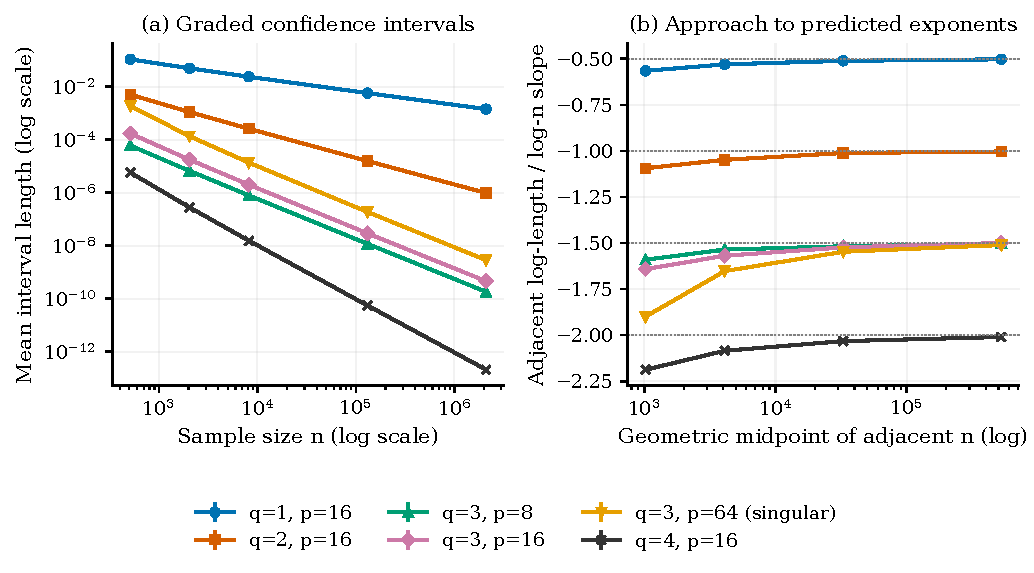
\includegraphics[width=\textwidth]{rates.pdf}
\caption{The graded interval exhibits contact orders one through four, with visible finite-dimension effects before the limiting regime. Each point uses 2,000 Gaussian datasets, $B_0=3E_{00\cdots0}$ and $A=E_{11\cdots1}$; mean-length bars are $\pm1.96$ Monte Carlo standard errors, often smaller than markers. The final two sample sizes are the disclosed addendum, and dotted slope guides mark $-q/2$.}\label{fig:rates}
\end{figure}

All graded intervals in the exactly specified contact experiments cover their targets. This demonstrates substantial conservatism. For example, at $n=2048$ in the four-way three-block setting, the mean graded length is $1.746\times10^{-5}$, compared with $1.741\times10^{-2}$ for the ambient scalar interval and $1.704\times10^{-8}$ for boundary-degree Wald. The last interval has empirical coverage 0.947 at the exact point but is not honest over its neighborhood. These numbers demonstrate a rate gain over ambient inference, not sharp constants or dominance over other valid minimum-distance constructions. In the $q=1$ slack setting, the graded ball is wider than the efficient scalar baseline.

\subsection{Rank activation and two prespecified functionals}
Use the path $B_{n,c}$ from Proposition~\ref{prop:wald}, with $c\in\{0,1,2,4,8\}$, $\lambda=3$ and $\sigma=0.2$. Its second central unfolding singular value is
\[
 \tau_2=\lambda|u_n|(1+u_n^2)
\]
for the values used here. It is zero at the boundary and is the smaller nonzero central singular value for $c>0$. The fixed loadings are
\[
 A_{\rm tan}=\frac{E_{0000}+0.35E_{0110}}{\sqrt{1+0.35^2}},
 \qquad A_{\rm normal}=E_{1111}.
\]
The first is substantially tangent aligned; the second is cubic normal at $c=0$ and nearly normal along the local path. Known-rank Wald uses an original-mode rank-one HOSVD when $c=0$ and the three-block HOSVD when $c>0$. Selected-rank Wald uses the former unless the second central singular value of OLS exceeds $\kappa\sigma\sqrt{2/n}$, with prespecified $\kappa=1,2,3$. These are diagnostic rank selectors, not asserted consistent selectors in a local-signal regime.

At $n=2048,c=2$, normal-loading coverage is 1.000 for graded inversion, 0.849 for known-rank Wald, 0.5525 for selected-rank Wald with $\kappa=2$, and 0.475 for boundary-degree Wald. The last value has Monte Carlo standard error about 0.0112. At $c=0$, its coverage is 0.9535. At $c=8$, it is 0.488, consistent with the approximately 0.4865 iterated limit in Proposition~\ref{prop:wald}. Thus knowledge of the actual rank does not remove functional degeneracy, and exact-boundary calibration does not provide uniform inference. For the tangent loading at $c=2$, corresponding known-rank and selected-$\kappa=2$ coverages are 0.9475 and 0.9255, showing a smaller but visible selection effect.

\subsection{Approximate structure and sensitivity}
For the four-way cubic loading, let $s_n=\tn^3/\lambda^2$. The allowance grid is
\[
 \eta\in\{0,s_n,100s_n,10000s_n,\tn^2/\lambda,\tn\}.
\] We evaluate both $B_0$ and the admissible departure $B_0+\eta A$, comparing exact-model and tube-aware graded intervals. At $n=2048$, $s_n=9.591\times10^{-9}$. A departure $\eta=\tn^2/\lambda=6.510\times10^{-6}$ reduces exact-model graded coverage to 0.847; tube-aware coverage is 1.000. At $\eta=10000s_n$, the exact-model interval has zero empirical coverage, while the tube-aware interval again covers in all replications and increases its mean length to $2.092\times10^{-4}$.

The honest interval's large finite-sample constants delay the visible transition relative to the asymptotic threshold $s_n$. It still covers all tested departures at $100s_n$ even though its exact-model guarantee does not apply there. This is consistent with a rate theorem whose constants are not sharp. Figure~\ref{fig:tube} shows both the cost of a known allowance at the exact point and the coverage consequence of ignoring a departure.

\begin{figure}[t]
\centering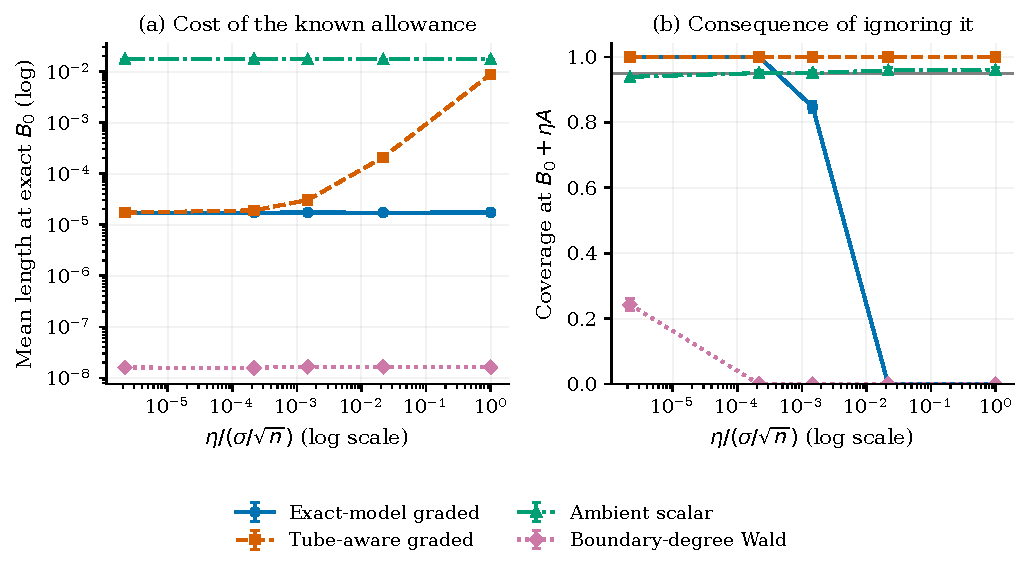
\includegraphics[width=\textwidth]{tube.pdf}
\caption{A known structural allowance increases honest length and protects against departures that invalidate exact-model inference. Four binary modes have caps $(1,2,1)$, $n=2048$, $\lambda=3$, $\sigma=0.2$, and $A=E_{1111}$. The left panel evaluates length at $B_0$ and the right coverage at $B_0+\eta A$, each with 2,000 replications; length bars are $\pm1.96$ Monte Carlo standard errors and coverage bars are Wilson 95\% Monte Carlo intervals.}\label{fig:tube}
\end{figure}

\subsection{Unknown noise, dense signals, and assumption diagnostics}
The study also varies $\lambda\in\{0.5,1,3\}$, rotates the signal and loading densely within modes, uses Gaussian design covariance $\Sigma_{ij}=0.5^{|i-j|}$, and evaluates the residual-$F$ procedure. The latter retains exact conditional coverage under Gaussian homoskedastic errors; a correlated full-rank design does not invalidate that statement. Dense rotations illustrate that coefficient sparsity is not needed.

Separate stress cases use standardized $t_5$ errors, heteroskedastic Gaussian errors, AR(1) errors with correlation 0.6, and Gaussian scale mixtures with 1\% or 5\% outlier probability and outlier standard deviation $5\sigma$. These cases are outside the exact noise theorem. For instance, at 5\% contamination the ambient interval using the uncontaminated $\sigma$ covers only 0.8045, while its residual-$t$ version covers 0.947 in this experiment. Conservative graded coverage at the tested boundary does not establish robustness to any of these departures. All diagnostic results, rather than only favorable settings, are included in the companion tables.

\section{Discussion and limitations}
The main conclusion is a classification of functional contact at original-mode rank-one points in capped TT classes. Cap-one cuts determine the exponent, while internal constraints can leave a singular feasible set without changing that exponent. If every cut permits an additional rank, all nonzero linear functionals return to first order. These statements describe the geometry of the declared class, not a universal benefit of tensor parameterization or rank selection.

The approximation result is consequential for interpretation. A confidence interval with an $n^{-3/2}$ pointwise length relies on a structural allowance of the same order if that gain is to persist uniformly. An ambient coefficient departure of order between $n^{-3/2}$ and $n^{-1/2}$ can be statistically undetectable and still dominate the target uncertainty. The theorem therefore argues for explicit sensitivity analysis whenever rank restrictions are approximate. It does not provide a way to infer the required small allowance from the same sample without additional assumptions.

The limitations are substantial. The pointwise length theorem fixes ambient dimension and the signal directions, with an original-mode rank-one evaluation point. The OLS ball can incur large dimension constants, and the experiments show that the computable interval is far from a sharp constant procedure. No matching dimension-dependent minimax length, efficient confidence constant, or general classification at non-rank-one TT points has been established. The inherited hardness of an exact local coefficient does not establish hardness of statistically optimal inference.

\paragraph{Status of possible extensions.}
\textsc{Partial}: growing-dimensional inference has a valid ambient localization construction and fixed-geometry lower bounds, but their dimension factors do not match. \textsc{Conjectured}: a general classification at non-rank-one points with several weak bonds may require higher-order feasible arcs beyond the present elementary paths; no universal rate is asserted. \textsc{Partial}: the spectral-norm reduction identifies a difficult constant but leaves computationally optimal intervals unresolved. \textsc{Conjectured}: non-Gaussian or dependent-noise versions would need new honest localization and moment bounds. These statements are research questions, not theorems of this paper.

\subsection{Relevance to modern AI and why no LLM benchmark is claimed}
A tensor regression head on frozen features offers a direct statistical setting for coefficient functionals. In a locally linear adapter model, a fixed evaluation contrast has the form $\ip{A}{B}$, with $A$ determined by held-out or externally fixed Jacobian features. Existing TT adapters make such restrictions plausible modeling choices, but a trained LLM does not automatically satisfy isotropic design, Gaussian residuals, fixed dimensions, or a known approximation allowance. A fully observed checkpoint is also a deterministic approximation object, not the sampling experiment in \eqref{eq:model}.

Accordingly, this draft contains no real-data or trained-LLM result. The companion application protocol specifies a frozen-feature regression study with a separately fixed functional, sample splitting for any learned loading, residual checks, and an explicit sensitivity grid. A convincing application would need to justify the population target and structural approximation bound, rather than add an LLM benchmark to support a general mathematical claim. The present theory applies independently of any AI interpretation.

\paragraph{Research assessment.}
The completed fixed-dimensional results support a focused theoretical manuscript for further expert evaluation. The central novelty candidate is the cap-profile classification and its inferential interpretation, not generic higher-order asymptotics. A broader theory of local moduli at singular structured parameters, or dimension-dependent optimality with a useful procedure, would be needed to make a strong case for the Annals of Statistics. The current draft should not be treated as submission ready solely because its proofs and experiments are complete.

\paragraph{Reproducibility and proof status.}
The accompanying project includes the full literature matrix, theorem ledger, assumption audit, canonical proof source, fixed-seed simulation code, replicate outputs, vector figures, and a workbook containing the plotted summaries and source metadata. Results marked \pr\ have complete derivations and internal mathematical checks. This label does not certify priority or replace independent mathematical review. The empirical addendum and the later supporting local-Wald derivation are disclosed in the project records.

\clearpage
\bibliography{references}
\clearpage
\appendix
\section{Complete derivations}\label{app:proofs}
Throughout, finite-dimensional norms are Euclidean or Frobenius. Every constant is allowed to depend on the fixed geometry specified in the theorem. The label \pr\ records a complete internal derivation, not independent peer review, a computer-verified proof, or a priority certificate.

\subsection{Product structure at cap-one cuts}
\begin{lemma}\label{lem:blocks}
Every nonzero tensor obeying the cap-one prefix constraints is a product across the induced consecutive blocks. Conversely, if a product of block tensors has within-block TT ranks at most the corresponding internal caps, it belongs to the full capped TT class whenever its norm is at most $M$.
\end{lemma}
\begin{proof}
At the first cap-one cut, a nonzero rank-one unfolding factors as a vector for the first block times a vector for the remaining modes. A later prefix unfolding is, up to row ordering, the Kronecker product of the first vector and the corresponding prefix unfolding of the remaining tensor. Multiplication by a nonzero vector preserves rank. The next cap-one constraint therefore factors the remaining tensor again. Induction proves the first assertion. The same rank-preservation calculation shows that an internal unfolding of a block product has the rank of that block's internal unfolding; a block boundary has rank one. This proves the converse. Zero belongs to both classes separately.
\end{proof}

\subsection{Proof of Theorem~\ref{thm:contact}}
Let $B=s\bigotimes_j w_j$ be a feasible nonzero tensor with unit block factors and $\norm{B-B_0}\le t$. Projecting $B_0-B$ orthogonally to the line spanned by $w_j$ in block $j$ gives
\[
 \lambda\sqrt{1-(v_j^\top w_j)^2}\le t.
\]
Consequently its component on the true block mask $S$ satisfies
\begin{equation}\label{eq:componentupper}
 \norm{B_S}\le(\lambda+t)(t/\lambda)^{|S|}.
\end{equation}
For $q\ge2$, all loading components of degree below $q$ vanish, as does $\ip{A}{B_0}$. Orthogonality, Cauchy--Schwarz, and \eqref{eq:componentupper} yield
\[
 |\ip{A}{B-B_0}|\le
 \sum_{|S|\ge q}\norm{A_S}(\lambda+t)(t/\lambda)^{|S|}
 \le 2^{J+1}\norm{A}\,t^q/\lambda^{q-1}
\]
when $t\le\lambda$. For $q=1$, ordinary Cauchy--Schwarz gives $\norm{A}t$. If $t\ge\lambda$, $\norm{A}t\le\norm{A}t^q/\lambda^{q-1}$, so the asserted global upper bound follows. Zero creates no exception, since it cannot be within $t<\lambda$ and is covered by Cauchy--Schwarz otherwise.

For the lower bound, first suppose $A_\varnothing\ne0$. The radial path $(\lambda+s)\bigotimes_jv_j$ is feasible for $|s|$ small, and its target change is a nonzero constant times $s$. Now suppose the minimum nonzero degree is $q\ge1$. Choose a mask $S$ of cardinality $q$ with $A_S\ne0$. Extend each original-mode signal factor to an orthonormal basis. The elementary basis products on each active block except its all-signal vector form an orthonormal basis for $v_j^\perp$. Thus some coefficient
\[
 c_A=\left\langle A,\bigotimes_{j\in S}w_j\bigotimes_{j\notin S}v_j\right\rangle
\]
is nonzero, with each $w_j$ an elementary original-mode product perpendicular to $v_j$. Consider
\[
 B(s)=\lambda\bigotimes_{j\in S}(v_j+s w_j)
                \bigotimes_{j\notin S}v_j.
\]
Within each active block this is the sum of two original-mode rank-one products, so every internal unfolding has rank at most two. Internal caps are at least two by construction; the boundary cuts have rank one. Lemma~\ref{lem:blocks} establishes feasibility. All terms of degree less than $q$ pair to zero with $A$, and there are no higher-degree terms. Therefore
\[
 \ip{A}{B(s)-B_0}=\lambda c_A s^q,\qquad
 \norm{B(s)-B_0}^2=\lambda^2\{(1+s^2)^q-1\}.
\]
Taking $s^2=(1+t^2/\lambda^2)^{1/q}-1$ gives the lower bound, since $s/(t/\lambda)\to q^{-1/2}$. The norm is $\sqrt{\lambda^2+t^2}<\lambda+t<M$.

For the exact elementary coefficient, use a local product chart for any feasible $B$ within $t<\lambda$:
\[
 B=c\bigotimes_{j=1}^J(v_j+z_j),\quad z_j\perp v_j,
 \quad c=\ip{B}{\bigotimes_jv_j}\ge\lambda-t>0.
\]
Nonzero projections onto every $v_j$ follow from the same positive $c$. Orthogonal expansion gives
\[
 t^2\ge(c-\lambda)^2+c^2\left\{\prod_j(1+\norm{z_j}^2)-1\right\}
 \ge c^2\sum_j\norm{z_j}^2.
\]
For the elementary loading active on $S$, its target is $c\prod_{j\in S}\ip{w_j}{z_j}$. Cauchy--Schwarz and the arithmetic--geometric mean inequality give
\[
 |\ip{A}{B}|\le c\prod_{j\in S}\norm{z_j}
 \le\frac{t^q}{q^{q/2}c^{q-1}}
 \le\frac{t^q}{q^{q/2}(\lambda-t)^{q-1}}.
\]
The previous path with $c_A=1$ has the matching leading coefficient. For $q=1$ it also attains the exact Cauchy--Schwarz bound $t$. This proves every claim of the theorem.

\subsection{Proof of Proposition~\ref{prop:slack} and the singular example}
Choose a unit elementary original-mode product $H$ with $\ip{A}{H}\ne0$, which exists because elementary products span the ambient space. Rank subadditivity gives
\[
 \rank((B+sH)^{[k]})\le\rank(B^{[k]})+1\le\bar r_k.
\]
For $|s|<M-\norm{B}$ the norm constraint also holds. This gives the lower bound $|\ip{A}{H}|t$; Cauchy--Schwarz gives the upper bound.

In the six-mode example, the middle block has dimensions $2\times2\times2\times2$. The internal edge unfoldings have rank at most two automatically. Its central $4\times4$ unfolding is constrained to rank at most two, a proper determinantal variety. At a rank-one point this variety is singular: the differentials of all its $3\times3$ minors vanish, so its algebraic tangent space is the full 16-dimensional space, whereas the dimension of the rank-at-most-two variety is $2(4+4-2)=12$. Factoring the two external nonzero lines gives a local product chart with this variety; its singularity persists. The elementary path in the preceding proof remains feasible and gives cubic contact. For any one prefix cut with cap one, the corresponding elementary contrast is perpendicular on both matrix sides and the two-factor calculation gives order two. At the other cuts cap two leaves rank-one slack, giving order one. This verifies the stated scope of the matrix comparison.

\subsection{Information bound and tube geometry}
\begin{lemma}[Two-point expected-length bound]\label{lem:twopoint}
If an interval has coverage at least $1-\alpha$ at $B_0$ and $B_1$, then
\[
 \E_{B_0,\sigma}|I|\ge|\ip{A}{B_1-B_0}|
 \left[1-2\alpha-\frac{\sqrt n\norm{B_1-B_0}}{2\sigma}\right]_+.
\]
\end{lemma}
\begin{proof}
The design distributions are identical at the two coefficients. Conditional Gaussian relative entropy equals $\norm{X(b_1-b_0)}^2/(2\sigma^2)$; its expectation under isotropic design is $n\norm{b_1-b_0}^2/(2\sigma^2)$. Pinsker's inequality therefore bounds total variation by $\sqrt n\norm{b_1-b_0}/(2\sigma)$. Under $B_0$, the event that the interval contains both target values has probability at least $1-2\alpha-\TV$. On that event its length is at least their separation. Integrating proves the bound. This is the usual two-point modulus argument, not a new information inequality.
\end{proof}

For a unit loading, compactness of $\Th_0$ and Cauchy--Schwarz give the tube sandwich, for small $t$ with $\lambda+t<M$:
\begin{equation}\label{eq:tubesandwich}
 \max\{\omega_{A,0}(t),\eta\wedge t\}
 \le\omega_{A,\eta}(t)
 \le\min\{t,\eta+\omega_{A,0}(t+\eta)\}.
\end{equation}
Indeed $\Th_0\subseteq\Th_\eta$ and $B_0+(\eta\wedge t)A$ supplies the two lower bounds. For any feasible $B$, choose a nearest $B^\dagger\in\Th_0$. Then $\norm{B-B^\dagger}\le\eta$ and $\norm{B^\dagger-B_0}\le t+\eta$, proving the upper bound. For a nonunit loading the corresponding factors are $\norm{A}$, which are absorbed in constants. If $\eta\le t$, Theorem~\ref{thm:contact} and $(t+\eta)^q\le2^qt^q$ give an upper bound of order $\eta+t^q/\lambda^{q-1}$. If $\eta>t$, use the upper bound $t$. The lower bounds combine via $\max(x,y)\ge(x+y)/2$.

Take $h=1-2\alpha>0$ and $t=h\tn$ in Lemma~\ref{lem:twopoint}. Its bracket is at least $h/2$. A supremizing local alternative, or a sequence approaching the supremum, gives the lower bound in Theorem~\ref{thm:length}, using \eqref{eq:tubesandwich}. The signal condition ensures these alternatives stay within the norm cap. For unknown $\sigma$, restricting the honest procedure to alternatives with this same $\sigma$ proves exactly the same lower bound. At a slack point Proposition~\ref{prop:slack} and the same lemma give a root-$n$ lower bound, matched by ambient inference.

For Corollary~\ref{cor:pretest}, the explicit alternative is within $\eta_n$ of $B_0$ and its norm is below $M$ eventually. The entropy calculation yields $\KL=\eta_n^2/(2\tn^2)\to0$, while its target separation is $\eta_n$. Apply the two-point bound. The argument applies to any measurable interval, including those obtained after an arbitrary rank pretest.

\subsection{Localization and moment control}
\begin{lemma}[Gaussian OLS localization]\label{lem:OLS}
Both radii in Section~\ref{sec:method} give conditional coverage at least $1-\alpha$ when $X$ has full column rank. Under isotropic Gaussian design, for fixed $p,J,\alpha$ and $n\ge2p+2J+8$, for every integer $1\le k\le\max(J,2)$,
\[
 \E\norm{z-b}^k+\E e^k\le C_k(\sigma/\sqrt n)^k.
\]
\end{lemma}
\begin{proof}
Conditional on $X$, $S^{1/2}(z-b)/\sigma$ is standard normal, and hence $\norm{z-b}^2\le\sigma^2\chi_p^2/\lambda_{\min}(S)$ under a coupling. The squared residual norm divided by $\sigma^2$ is independent $\chi^2_{n-p}$ by orthogonal Gaussian projections. The normalized squared Mahalanobis error divided by $p\widehat\sigma^2$ is therefore $F_{p,n-p}$. These facts prove both coverage statements.

Here are details ensuring the expectation bound does not discard a localization failure event. Write $S=X^\top X\sim W_p(n,I)$. The reciprocal of $(S^{-1})_{jj}$ is the squared norm of column $j$ after projecting off the other $p-1$ columns. Conditioning on those columns shows it has law $\chi^2_{\nu}$, $\nu=n-p+1$. For $a>0$ with $\nu>2a$,
\[
 \E(\chi_\nu^2)^{-a}=2^{-a}\frac{\Gamma(\nu/2-a)}{\Gamma(\nu/2)}.
\]
For fixed $a$ and $\nu\ge2a+2$, this is at most $C_a\nu^{-a}$: the gamma-ratio asymptotic proves boundedness after multiplication by $\nu^a$ at infinity, and continuity bounds it on the remaining closed interval. This use of the gamma ratio involves fixed moment order only. Since $\lambda_{\min}(S)^{-1}\le\operatorname{tr}(S^{-1})$, for $a\ge1$ the inequality $(\sum_jx_j)^a\le p^{a-1}\sum_jx_j^a$ gives
\[
 \E\lambda_{\min}(S)^{-a}\le C_{a,p}n^{-a}.
\]
For $0<a<1$, Jensen's inequality and $\E\operatorname{tr}(S^{-1})=p/(n-p-1)$ give the same conclusion. Conditional Gaussian moments now bound $\E\norm{z-b}^k$ by $C_{k,p}\sigma^k\E\lambda_{\min}(S)^{-k/2}$.

The residual scale has $k$th moment bounded by $C_k\sigma^k$, uniformly in $n-p\ge1$, and is independent of $S$ since its conditional distribution does not depend on $X$. The fixed upper quantiles $F_{p,n-p;1-\alpha}$ are bounded over integers $n-p$ bounded away from zero: their distributions converge to $\chi_p^2/p$, and the finite initial set has finite quantiles. Thus the known- and unknown-noise radii have the asserted moment bounds. The displayed sample-size condition is sufficient for all these inverse moments; it is not claimed necessary.
\end{proof}

\begin{lemma}[HOSVD pilot and changing block projectors]\label{lem:pilot}
Let $\widehat B$ be the rank-one HOSVD approximation to $Z$. For every block-product $B_0$,
\[
 \norm{Z-\widehat B}\le\sqrt J\norm{Z-B_0},\qquad
 h:=\norm{\widehat B-B_0}\le(1+\sqrt J)\norm{Z-B_0}.
\]
If $h<\lambda/2$ and $A$ has no true block components of degree below $q\ge1$, then
\begin{equation}\label{eq:mixing}
 \norm{\widehat\Pi_\ell A}\le C_J\norm{A}
 (h/\lambda)^{(q-\ell)_+},\qquad 0\le\ell\le J.
\end{equation}
For $q=1$ with a radial loading component, only the trivial bounds needed below are asserted.
\end{lemma}
\begin{proof}
Let $\widehat P_j$ be the leading left-singular-vector projection in mode $j$. It minimizes the mode-$j$ rank-one projection residual, which is at most $\norm{Z-B_0}$ because the true block line is an admissible competitor. The commuting orthogonal projections have the telescoping expansion
\[
 Z-\prod_j\widehat P_j Z
 =\sum_j\left(\prod_{i<j}\widehat P_i\right)(I-\widehat P_j)Z.
\]
Terms are orthogonal: for terms $j<k$, the first lies in the complement of the $j$th line and the second lies in that line. Summing squared norms proves the first bound; the triangle inequality proves the second.

Projection of $B_0-\widehat B$ off the pilot line in block $j$ gives $\lambda\sin\theta_j\le h$. The two cross-line operators satisfy $\norm{\widehat P_jQ_j}_{\rm op}=\norm{(I-\widehat P_j)P_j}_{\rm op}=\sin\theta_j$. If a true mask $S$ has size at least $q$ and a pilot mask $T$ has size $\ell<q$, then $|S\setminus T|\ge q-\ell$. The tensor product of mask operators therefore has operator norm at most $(h/\lambda)^{q-\ell}$; all other factors have norm at most one. Sum over the at most $2^{2J}$ pairs of masks and use $\sum_S\norm{A_S}\le2^{J/2}\norm{A}$. For $\ell\ge q$, use the contractivity of an orthogonal projection. These steps establish \eqref{eq:mixing} with a finite $J$-dependent constant.
\end{proof}

\subsection{Proof of Theorem~\ref{thm:procedure}}
On the OLS ball event, take a closest $B^\dagger\in\Th_0$ to the true $B\in\Th_\eta$. Compactness ensures existence, and
\[
 \norm{B^\dagger-\widehat B}\le\eta+\norm{B-z}+\norm{z-\widehat b}\le\rho.
\]
By Lemma~\ref{lem:blocks}, $B^\dagger$ is in the block-product envelope. If $\rho<\widehat s/2$, write it in the pilot chart as $c\bigotimes_j(\widehat v_j+z_j)$, where $z_j\perp\widehat v_j$ and $c\ge\widehat s-\rho>0$. Its orthogonal expansion implies $c\norm{z_j}\le\rho$ for each $j$. For every mask $S$ of size $\ell\ge2$,
\[
 \norm{(B^\dagger)_S}=c\prod_{j\in S}\norm{z_j}
 \le\rho^\ell/c^{\ell-1}.
\]
The components are orthogonal, so their combined norm is bounded by $\binom{J}{\ell}^{1/2}\rho^\ell/(\widehat s-\rho)^{\ell-1}$. The degree-zero and degree-one part of $B^\dagger-\widehat B$ has norm at most $\rho$. Pairing with the corresponding loading projections proves the second expression in \eqref{eq:graded}; Cauchy--Schwarz proves the first. The fallback is valid for the same reason. The difference between the true and projected targets is at most $\eta\norm{A}$. Thus $I_s$ contains the true target on the ball event. So does $I_a$. Their intersection is nonempty and contains it on that event. This proves conditional coverage, without any independence between pilot and ball.

It remains to prove expected length, not merely length on a favorable event. At $B_0$, put $r=\norm{z-b_0}$ and $T=r+e$. Lemma~\ref{lem:pilot} gives
\[
 h\le(1+\sqrt J)r,\quad \norm{z-\widehat b}\le\sqrt J r,
 \quad\rho\le(1+\sqrt J)(T+\eta).
\]
First let $\eta\le\tn$. Choose a fixed small $c_J>0$ so that on $G=\{T+\eta\le c_J\lambda\}$, $h\le\lambda/8$, $\rho\le\lambda/8$, and $\widehat s-\rho\ge3\lambda/4$. When $q\ge2$, \eqref{eq:mixing} bounds the first part of \eqref{eq:graded} by
\[
 C\norm{A}(h/\lambda)^{q-1}\rho
 \le C\norm{A}(T+\eta)^q/\lambda^{q-1}.
\]
For $2\le\ell<q$, the same inequality bounds its $\ell$th summand by
\[
 C\norm{A}(h/\lambda)^{q-\ell}\rho^\ell/\lambda^{\ell-1}
 \le C\norm{A}(T+\eta)^q/\lambda^{q-1}.
\]
For $\ell\ge q$, use $\rho/\lambda\le1$ to reach the same bound. For $q=1$ use $H\le\norm{A}\rho$ directly, including a nonzero radial component. Thus on $G$, $H\le C\norm{A}(T+\eta)^q/\lambda^{q-1}$.

On $G^c$ the definition always gives $H\le\norm{A}\rho\le C\norm{A}(T+\eta)$. Moreover
\[
 (T+\eta)\one_{G^c}\le
 \frac{(T+\eta)^q}{(c_J\lambda)^{q-1}},
\]
also for $q=1$. Lemma~\ref{lem:OLS}, $\eta\le\tn$, and $(x+y)^q\le2^{q-1}(x^q+y^q)$ now yield
\[
 \E|I|\le2\eta\norm{A}+2\E H
 \le C\{\eta+\tn^q/\lambda^{q-1}\}.
\]
If $\eta>\tn$, intersection with $I_a$ gives $|I|\le2e\norm{A}$ (the empty case has zero length), so its expectation is at most $C\tn$. This proves the assertion for every $\eta$. Together with the two-point lower bound it completes Theorem~\ref{thm:length}.

\subsection{Proof of Proposition~\ref{prop:hardness}}
In the local chart $B=c(e_0+x)\otimes(e_0+y)\otimes(e_0+z)$, each vector is perpendicular to $e_0$. The target equals $c\ip{T}{x\otimes y\otimes z}$. The energy bound gives $c^2(\norm{x}^2+\norm{y}^2+\norm{z}^2)\le t^2$. Hence
\[
 |\ip{A}{B}|\le c\norm{T}_{\rm inj}\norm{x}\norm{y}\norm{z}
 \le\frac{\norm{T}_{\rm inj}t^3}{3\sqrt3(\lambda-t)^2}.
\]
Compactness of the unit spheres gives maximizing directions for $\norm{T}_{\rm inj}$. The product path with those directions and $s^2=(1+t^2/\lambda^2)^{1/3}-1$ is feasible in the three-block product class and attains the matching limit. Setting $\lambda=1$ identifies the squared spectral norm with 27 times the squared modulus coefficient. Thus an oracle evaluating this coefficient exactly also evaluates a known NP-hard tensor quantity as dimensions vary. The reduction adds no claim about approximation factors beyond those established for that source problem.

\subsection{Proof of Proposition~\ref{prop:wald}}
Under the triangular sequence $B_{n,c}$, the OLS error distribution is independent of the coefficient. The law of large numbers gives $S/n\to I$ in probability, and conditional normality implies
\[
 (z-b_{n,c})/\tn\xrightarrow{d}G,\qquad G\sim N_p(0,I).
\]
This implication can be verified directly from conditional characteristic functions:
\[
 \E[\exp\{-h^\top(nS^{-1})h/2\}]\to\exp(-\norm{h}^2/2),
\]
by bounded convergence in probability. Expand $B_{n,c}=B_0+c\tn\sum_{j=1}^3 E_j+O(\tn^2/\lambda)$, where $E_j$ changes the designated coordinate in exactly block $j$. These three elementary tensors are orthonormal.

For completeness, the required HOSVD first-order expansion follows from its eigenvector equation. In any block unfolding, $Z=\lambda e_0w_0^\top+\tn D_n$, with $D_n=O_P(1)$, so
\[
 ZZ^\top=\lambda^2e_0e_0^\top+
 \lambda\tn(e_0g_n^\top+g_ne_0^\top)+O_P(\tn^2),\quad g_n=D_nw_0.
\]
Weyl's bound, obtained here from the Rayleigh variational formula, places the largest eigenvalue at $\lambda^2+O_P(\tn)$ and all other eigenvalues at $O_P(\tn)$. Choose the leading unit eigenvector with positive first coordinate, and write it $a_ne_0+h_n$, $h_n\perp e_0$. Projecting its eigenvector equation orthogonally to $e_0$ first gives $h_n=O_P(\tn/\lambda)$, then substitution gives
\[
 h_n=(\tn/\lambda)(I-e_0e_0^\top)g_n+O_P(\tn^2/\lambda^2),
 \qquad a_n=1+O_P(\tn^2/\lambda^2).
\]
Indeed the projected linear operator on $h_n$ has inverse norm $O_P(\lambda^{-2})$, and the cross block is $\lambda\tn(I-e_0e_0^\top)g_n+O_P(\tn^2)$, which justifies both substitutions. The HOSVD scalar coefficient equals $\lambda+O_P(\tn)$. The designated perpendicular coordinate in block $j$ therefore equals $(\tn/\lambda)(c+Z_{n,j})+o_P(\tn/\lambda)$, where jointly $Z_{n,j}\to Z_j$ and their independence follows from the orthonormal $E_j$ coordinates of $G$.

Contracting the pure-normal loading with the fitted product yields the asserted product limit. For its tangent projection, the leading terms are the three mutually orthogonal $E_j$ directions, with coefficients
\[
 (\tn/\lambda)^2\prod_{k\ne j}(c+Z_{n,k})+o_P(\tn^2/\lambda^2).
\]
The radial term is of order $(\tn/\lambda)^3$; perturbing the remaining unit directions changes the leading terms only by a smaller order. Since $nS^{-1}\to I$, the standard-error limit follows.

The limiting denominator is positive almost surely. The equality boundary of the coverage event has probability zero: after squaring, it is the zero set of a nonzero polynomial in a Gaussian vector. To see the latter fact without a regularity assumption, induct on dimension, condition on all but one coordinate, and use that a nonzero univariate polynomial has finitely many roots; the exceptional coefficient-zero sets are treated by the induction hypothesis. Thus convergence in distribution gives convergence of coverage probabilities. At $c=0$ apply the cited monomial law. Finally, as $c\to\infty$,
\[
 \frac{\prod_j(c+Z_j)-c^3}
 {\{\sum_j\prod_{k\ne j}(c+Z_k)^2\}^{1/2}}
 =\frac{Z_1+Z_2+Z_3}{\sqrt3}+o_P(1).
\]
This follows by dividing numerator and denominator by $c^2$ and expanding the finite products. The displayed iterated limits now follow from the standard normal distribution. No uniform-in-$c$ approximation or arbitrary growing-$c_n$ limit is asserted.

\end{document}
